\documentclass[12pt, a4paper]{article}
\usepackage[top=1.0in, bottom=1.0in, left=0.8in, right=0.8in]{geometry}

\setlength{\parskip}{\baselineskip}%
\setlength{\parindent}{0pt}%
\usepackage{bookmark}
\usepackage[]{graphicx}
\usepackage{enumitem}
\usepackage{amsmath}
\usepackage{relsize}
\usepackage{cprotect}
\usepackage{amsmath, amsfonts}
\usepackage{siunitx}
\usepackage{mathrsfs}
\usepackage{framed}
\usepackage{enumitem}
\usepackage{tikz}
\usepackage{circuitikz}
\usepackage{float}
\usepackage[english]{babel}
\usepackage{blindtext}

\newlist{notes}{enumerate}{1}
\setlist[notes]{label=\textbf{Note:} ,leftmargin=*}

\newlist{hints}{enumerate}{1}
\setlist[hints]{label=\textbf{Hint:} ,leftmargin=*}

\usepackage{xcolor}
\usepackage{color}
\definecolor{com1}{RGB}{125,125,125}
\definecolor{comment}{RGB}{140,115,115}
\definecolor{numbering}{rgb}{0.2,0.2,0.2}
\definecolor{key}{RGB}{0,0,180}
\definecolor{in}{RGB}{0,100,0}
\definecolor{out}{RGB}{100,30,30}
\definecolor{bg}{RGB}{245,245,245}
\definecolor{bgLight}{RGB}{250,250,250}
\definecolor{string}{RGB}{0,150,0}

\usepackage{hyperref}
\hypersetup{
    colorlinks=true,
    linkcolor=blue,
    filecolor=magenta,      
    urlcolor=blue,
}
\urlstyle{same}

\usepackage{listings}

\lstdefinestyle{py_code}{ %
    backgroundcolor=\color{bg},      % choose the background
    basicstyle=\ttfamily\small,		      % fonts
    breakatwhitespace=false,         % automatic breaks at whitespace ?
    breaklines=true,                 % sets automatic line breaking
    captionpos=b,                    % caption-position - bottom
    commentstyle=\itshape\color{comment},    % comment style
    extendedchars=true,              % use non-ASCII
    frame=single,	                   % single frame around the code
    keepspaces=true,                 % keeps spaces in text
    keywordstyle=\bfseries\color{key},% keyword style
    language=Python,                 	  % the language of the code
    morekeywords={Null},       % add more keywords to the set
    numbers=left,                    % line_numbers (none, left, right)
    numbersep=10pt,                  % line_no - code dist
    numberstyle=\footnotesize\color{numbering}, % line_no style
    rulecolor=\color{black},         % frame_color [!always set]
    showspaces=false,                % show spaces everywhere
    showstringspaces=false,          % 
    showtabs=false,                  % 
    stepnumber=1,                    % step b/w two line-no
    stringstyle=\color{string},     % string literal style
    tabsize=2,	                       % sets default tabsize to 2 spaces
    title=\lstname,                  % show the filename
    escapeinside={(*}{*)},			  % escape from style inside (* *)
    xleftmargin=\parindent,
    belowskip=-1.3 \baselineskip,
    aboveskip=1.0 \baselineskip,
    columns=fullflexible,
    xleftmargin=0.15in,
}
\lstnewenvironment{py_code}
{\lstset{style=py_code}}
{}

\lstdefinestyle{psudo}{ %
    backgroundcolor=\color{bgLight},   % choose the background
    basicstyle=\ttfamily\small,		      % fonts
    breakatwhitespace=false,         % automatic breaks at whitespace ?
    breaklines=true,                 % sets automatic line breaking
    captionpos=b,                    % caption-position - bottom
    commentstyle=\itshape\color{com1},          % comment style
    extendedchars=true,              % use non-ASCII
    keepspaces=true,                 % keeps spaces in text
    language=C,                 	  % the language of the code
    morekeywords={type,NULL, True, False},       % add more keywords to the set
    showspaces=false,                % show spaces everywhere
    showstringspaces=false,          % 
    showtabs=false,                  % 
    tabsize=2,	                       % sets default tabsize to 2 spaces
    title=\lstname,                  % show the filename
    escapeinside={(*}{*)},			  % escape from style inside (* *)
    belowskip=-1.8 \baselineskip,
    aboveskip=0.9 \baselineskip,
    columns=fullflexible,
    xleftmargin=0.2in,
    frame=tb,
    framexleftmargin=16pt,
    framextopmargin=6pt,
    framexbottommargin=6pt, 
    framerule=0pt,
}

\lstnewenvironment{psudo}
{\lstset{style=psudo}}
{}

\graphicspath{ ./ }

\title{\textbf{EE2703 : Applied Programming Lab \\ Assignment 5 \\ Laplace Equation}} 
\author{Chagari Koushal Kumar Reddy \\ EE20B023} % Author name

\date{\today} % Date for the report

\begin{document}		

\maketitle % Insert the title, author and date
\clearpage

\tableofcontents
\clearpage

\section{Aim}
The aim of this assignment is to :
\begin{itemize}
    \item Solve the Laplace equation of the electric potential ($\phi$) in a resistor and hence, find the current density distribution
    \item Analyze the potential, current and temperature profile of the resistor
    \item Apply the "Average of Neighbours" method to solve the Laplace equation and analyze the error present in the method
\end{itemize}

\section{Theory}
\subsection{The Resistor Problem}
Let us consider a copper plate of dimensions 1cm x 1cm with a wire soldered in the middle portion of the plate. Also the wire is maintained at a constant potential of 1 Volt.
The bottom edge of the plate is grounded and the remaining edges are floating.

\begin{figure}[H]
    \centering
    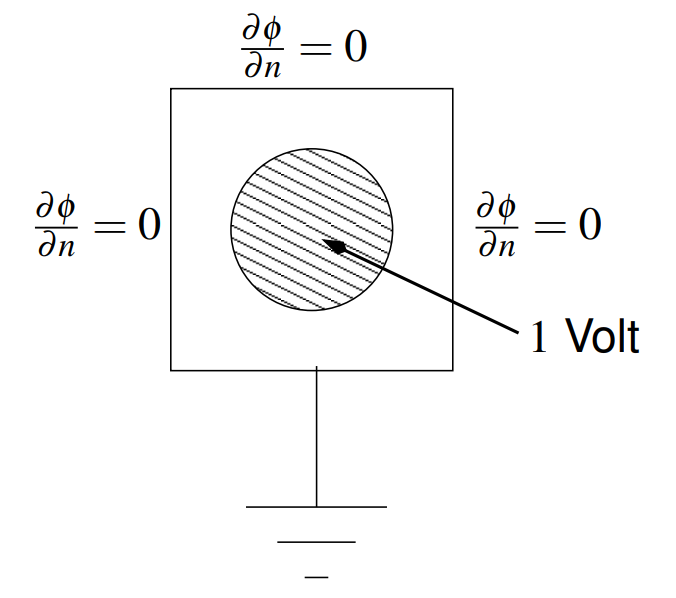
\includegraphics[scale = 0.6]{Figure_0.png}
\end{figure}
We have the following equations:
\vspace{-0.5cm}
\begin{enumerate}
    \item $\vec{j} = \sigma \vec{E}$ (Ohm's Law)
    \item $\vec{E} = -\nabla \phi$ (Field-Potential relation)
    \item $\nabla .\vec{j} = -\frac{\partial \rho}{\partial t}$ (Continuity equation)
\end{enumerate}
Combining these equations we have:
\begin{equation*}
    \nabla ^{2}\phi = 0  (Laplace equation)
\end{equation*}
\subsection{Solving the Laplace Equation}
For a 2-D surface, the Laplace equation can be written as:
\begin{equation*}
    \frac{\partial ^{2}\phi}{\partial x^{2}} + \frac{\partial ^{2}\phi}{\partial x^{2}} = 0
\end{equation*}
Assuming the neighbouring potential values are known, we can write:
\begin{equation*}
    \frac{\partial \phi}{\partial x} \bigg\rvert _ {(x_{i},y_{i})} = \frac{\phi (x_{i+1/2},y_{j}) - \phi (x_{i-1/2},y_{j})}{\Delta x}
\end{equation*}
and hence:
\vspace{0.2cm}
\begin{equation*}
    \frac{\partial ^{2}\phi}{\partial x^{2}} \bigg\rvert _ {(x_{i},y_{i})} = \frac{\phi (x_{i+1},y_{j}) - 2\phi (x_{i},y_{j}) + \phi (x_{i-1},y_{j})}{(\Delta x)^{2}}
\end{equation*}

Similarly for the partial derivative with respect to y:
\begin{equation*}
    \frac{\partial ^{2}\phi}{\partial y^{2}} \bigg\rvert _ {(x_{i},y_{i})} = \frac{\phi (x_{i},y_{j+1}) - 2\phi (x_{i},y_{j}) + \phi (x_{i},y_{j-1})}{(\Delta y)^{2}}
\end{equation*}

Assuming same in both the axes ($\Delta x = \Delta y$), we have:
\begin{equation*}
    \phi _{i,j} = \frac{\phi _{i+1,j} + \phi _{i-1,j} + \phi _{i,j+1} + \phi _{i,j-1}}{4}
\end{equation*}

This solution is called the \textbf{Average of Neighbours}. If there exists a discrete solution for this equation, then it should satisfy this relationship. So the method is clear.
We should guess a solution and carry out the averaging process until we reach a convergence point.

\subsection{Boundary Conditions}
The following boundary conditions should be followed:
\vspace{-0.3cm}
\begin{enumerate}
    \item The soldered wire is always maintained at a potential of 1 Volt. (The circular region in the middle)
    \item The bottom edge of the plate is grounded, which potential is 0 Volt there.
    \item The other 3 edges are floating and not connected to anything, which means the current at the edges must be parallel to the edges.
Hence the normal derivative of the potential($\frac{\partial \phi}{\partial n}$) is 0.
\end{enumerate}

\subsection{Current density distribution}
There will be a current flowing from the soldered wire to the grounded edge because of a potential drop. However the current distribution will be non-uniform due to non-uniform potential profile.
Current density (J) is given by:
\begin{equation*}
    \vec{J} = -\sigma (\nabla \phi)
\end{equation*}

Based on the formula we had for the partial derivatives we can write:
\begin{equation*}
    J_{x,ij} = \sigma \frac{\phi _{i,j-1} - \phi _{i,j+1}}{2 \Delta x}
\end{equation*}
\begin{equation*}
    J_{y,ij} = \sigma \frac{\phi _{i-1,j} - \phi _{i+1,j}}{2 \Delta x}
\end{equation*}

For simplicity let us assume $\sigma = \Delta x = \Delta y$, since the qualitative nature of current density plot doesn't depend on the value of the conductivity.
Hence we will have:
\begin{equation*}
    J_{x,ij} = \frac{\phi _{i,j-1} - \phi _{i,j+1}}{2}
\end{equation*}
\begin{equation*}
    J_{y,ij} = \frac{\phi _{i-1,j} - \phi _{i+1,j}}{2}
\end{equation*}

\subsection{Temperature profile}
Due to the currents present in the metal plate, Joule heating takes place. This heat increses the temperature of the plate. However the temperature of the plate won't be uniform.
Temperature (T) will satisfy the following equation:
\begin{equation*}
    \nabla .(\kappa \nabla T) = -\frac{1}{\sigma}|J|^{2}
\end{equation*}
Using the averaging technique we will have:
\begin{equation*}
    \frac{T(x_{i+1},y_{j}) - T(x_{i},y_{j}) + T(x_{i-1},y_{j})}{(\Delta x)^{2}} + \frac{T(x_{i},y_{j+1}) - T(x_{i},y_{j}) + T(x_{i},y_{j-1})}{(\Delta y)^{2}} = -\frac{1}{\kappa \sigma}|J|^{2}
\end{equation*}

From this we will have:
\begin{equation*}
    T_{i,j} = \frac{T_{i+1,j} + T_{i-1,j} + T_{i,j+1} + T_{i,j-1}}{4} + \frac{(\Delta x)^{2}}{4\kappa \sigma}|J|^{2}
\end{equation*}
We know from the previous section that $\sigma = \Delta x = \Delta y$. To simplify the equation let us also assume $\sigma = \kappa$. Hence we have:
\begin{equation*}
    T_{i,j} = \frac{T_{i+1,j} + T_{i-1,j} + T_{i,j+1} + T_{i,j-1}}{4} + \frac{1}{4}|J|^{2}
\end{equation*}
with J obtained from the gradient of the potential.

The boundary conditions of temperature are:
\begin{enumerate}
    \item The soldered wire is maintained at room temperature (300K).
    \item The grounded edge is maintained at room temperature (300K).
    \item The normal component of temperature gradient is 0 at the other 3 edges. 
    \item Initially the plate was at room temperature (300K).
\end{enumerate}
\section{Procedure}
\subsection{Variables used:}
\begin{enumerate}
    \item Nx = Number of X-axis divisions (No.of columns)
    \item Ny = Number of Y-axis divisions (No.of rows)
    \item radius = Radius of the central wire (In terms of number of units)
    \item Niter = Number of iterations till which the averaging process is done
\end{enumerate}
\subsection{Solving the Laplace Equation}
The potential profile is obtained using Averaging the Neighbours algorithm. This is the python code snippet I used:
\begin{py_code}
for k in range(Niter):
    oldphi = phi.copy()
    phi[1:-1,1:-1] = (0.25)*(oldphi[1:-1,0:-2] + oldphi[1:-1,2:] + oldphi[0:-2,1:-1] + oldphi[2:,1:-1])
    # Making the first column equal to the second column - do(phi)/do(x) = 0
    phi[:,0] = phi[:,1]
    # Making the last column equal to the last second column - do(phi)/do(x) = 0
    phi[:,-1] = phi[:,-2]
    # Making the first row equal to the second row so that do(phi)/do(y) = 0           
    phi[0,:] = phi[1,:]      
    # Reasserting the boundary condition that the middle circle is at 1V       
    phi[ii] = 1.0                   
    errors[k] = abs(phi - oldphi).max()
\end{py_code}
I used the following code to calculate the X, Y components of the current densities:
\begin{py_code}
    Jx = (0.5)*(phi[1:-1,0:-2] - phi[1:-1,2:])
    Jy = (0.5)*(phi[0:-2,1:-1] - phi[2:,1:-1])
\end{py_code}
\vspace{0.7cm}
I used the following code to calculate the temperature profile:
\begin{py_code}
    T = np.zeros((Ny,Nx)) + 300.0
    heats = np.multiply(Jx,Jx) + np.multiply(Jy,Jy)

    for k in range(Niter):
        T[1:Ny-1,1:Nx-1] = 0.25*( T[0:Ny-2,1:Nx-1] + T[2:Ny,1:Nx-1] + T[1:Ny-1,0:Nx-2] + T[1:Ny-1,2:Nx] + heats )
        T[0,:Nx] = 300.0
        T[:Ny,0] = T[:Ny,1]
        T[:Ny,Nx-1] = T[:Ny,Nx-2]
        T[Ny-1,:Nx] = T[Ny-2,:Nx]
        T[ii] = 300.0   
\end{py_code}
\subsection{Error Analysis}
At every iteration, the maximum absolute error between the new potential values and the old potential values is calculated and stored in an array named "errors".
The errors are plotted against the iteration using semilog and loglog plots. We observe that the semilog plot is linear after 500 iteration indicating that the error varies with the number of iterations as:
\begin{equation*}
    \log (errors_{k}) = \log (A) + Bk
\end{equation*}
Now we can fit (A,B) which satisfies the above equation. We have to find 2 fits:
\vspace{-0.3cm}
\begin{enumerate}
    \item Fit 1: Data corresponding to all iterations
    \item Fit 2: Data corresponding to all iterations excluding the first 500
\end{enumerate}
Writing the equation in matrix form, we have:
\begin{equation*}
    \begin{pmatrix}
        1 & 0 \\
        1 & 1 \\
        1 & 2 \\
        \ldots & \ldots \\
        1 & Niter - 2 \\
        1 & Niter - 1
    \end{pmatrix}
    \begin{pmatrix}
        A\\
        B
    \end{pmatrix}
    = \begin{pmatrix}
        \log (errors_{0}) \\
        \log (errors_{1}) \\
        \log (errors_{2}) \\
        \ldots \\
        \log (errors_{Niter - 2 }) \\
        \log (errors_{Niter - 1}) \\
    \end{pmatrix}
\end{equation*}

This equation is of the form:
\begin{equation*}
    Mx = y
\end{equation*}

For Fit 2, the matrix will start from 501. Now to solve for A, B we use the lstsq function of the numpy module. The following code snippet shows how the 2 fits are calculated:
\vspace{0.8cm}
\begin{py_code}
    x = np.arange(Niter)
    x.shape = (Niter,1)
    A = np.c_[np.ones((Niter,1)),x]
    b = np.log(errors)
    fit1 = np.linalg.lstsq(A,b,rcond = None)[0]
    fit2 = np.linalg.lstsq(A[500:],b[500:],rcond = None)[0]
\end{py_code}

\section{Observations and plots}
\subsection{Initial potential contour}
\vspace*{-0.5cm}
\begin{figure}[H]
    \centering
    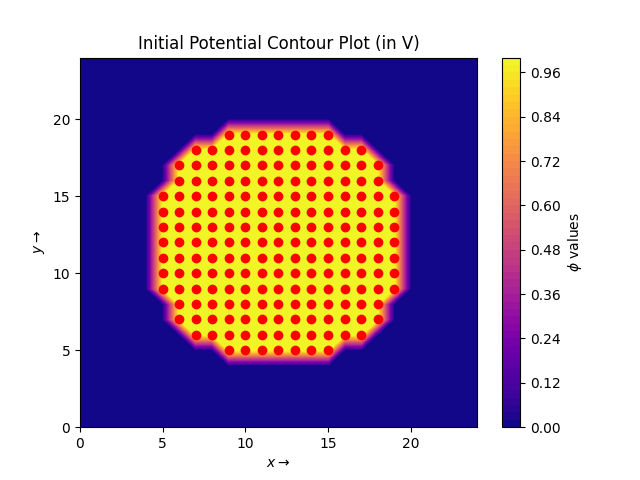
\includegraphics[scale = 0.75]{Figure_1.png}
    \label{fig:sample}
\end{figure}
\vspace*{-0.5cm}
\begin{center}
    Initially, the potential is zero at all points except the wire. The wire is at 1 Volt
\end{center}
\subsection{Semilogy plot of the Error vs Iteration number}
\vspace*{-0.5cm}
\begin{figure}[H]
    \centering
    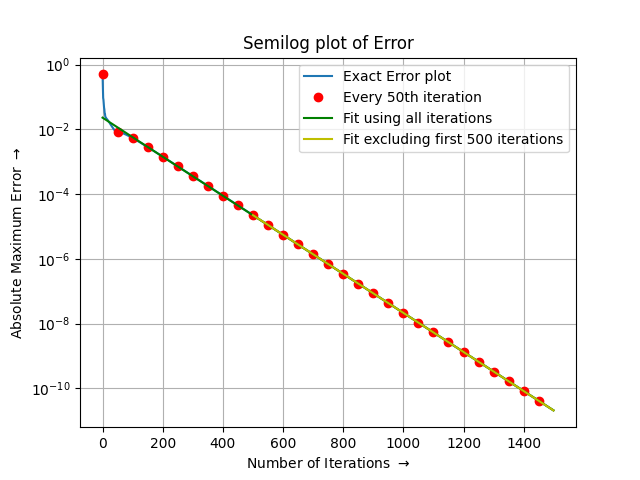
\includegraphics[scale = 0.75]{Figure_2.png}
    \label{fig:sample}
\end{figure}
\vspace*{-0.5cm}
\begin{center}
    The exact error is different from the fit for low values of iteration. However,
the fit is somewhat accurate for higher values of iteration
\end{center}
\subsection{Loglog plot of the Error vs Iteration number}
\vspace*{-0.5cm}
\begin{figure}[H]
    \centering
    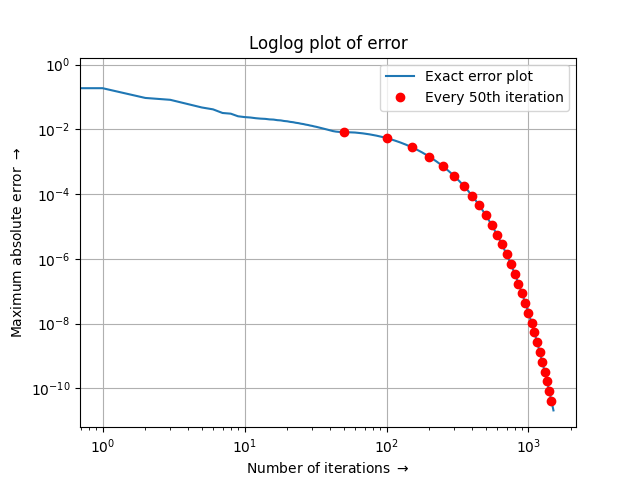
\includegraphics[scale = 0.75]{Figure_3.png}
    \label{fig:sample}
\end{figure}
\vspace*{-0.5cm}
\begin{center}
    On the loglog plot, the error is intially decreasing linearly with respect to the
iteration number. However, the plot reaches an exponential regime for higher
values of iteration
\end{center}
\subsection{3D Surface Potential Plot}
\vspace*{-0.5cm}
\begin{figure}[H]
    \centering
    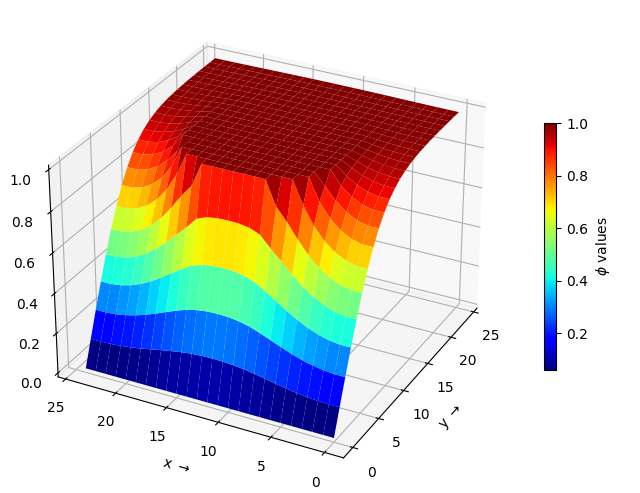
\includegraphics[scale = 0.75]{Figure_4.png}
    \label{fig:sample}
\end{figure}
\vspace*{-0.5cm}
\begin{center}
    The 2D contour matches with the 3D plot exactly and both the contours
follow the boundary conditions as well
\end{center}
\subsection{Final Potential Contour Plot}
\vspace*{-0.5cm}
\begin{figure}[H]
    \centering
    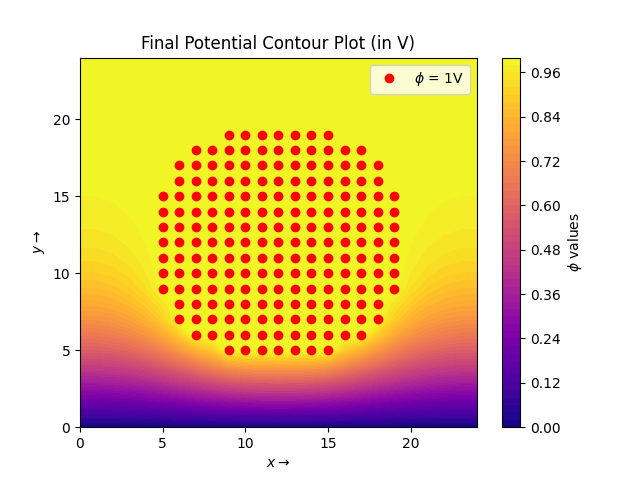
\includegraphics[scale = 0.75]{Figure_5.png}
    \label{fig:sample}
\end{figure}
\vspace*{-0.5cm}
\begin{center}
    After the averaging is done and the boundary conditions are satisfied, the
potential becomes much more smoother
\end{center}
\subsection{Vector plot of the current density}
\vspace*{-0.5cm}
\begin{figure}[H]
    \centering
    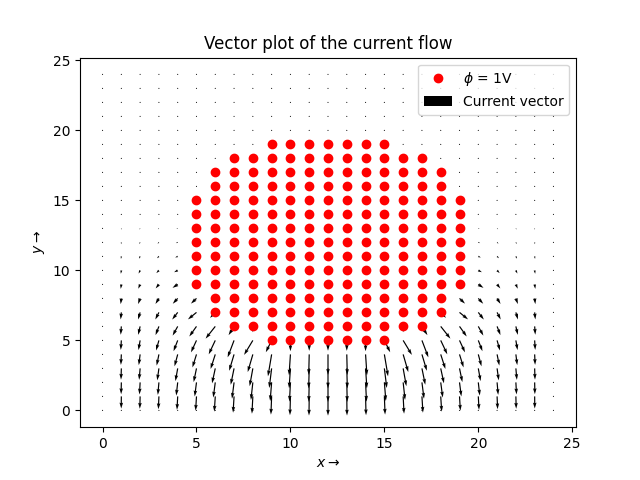
\includegraphics[scale = 0.75]{Figure_6.png}
    \label{fig:sample}
\end{figure}
\vspace*{-0.5cm}
\begin{center}
    As expected, the currents are only existing in the region between the wire and
the grounded edge. The current density values in the floating regions are
practically negligible
\end{center}
\subsection{Temperature Profile Contour}
\vspace*{-0.5cm}
\begin{figure}[H]
    \centering
    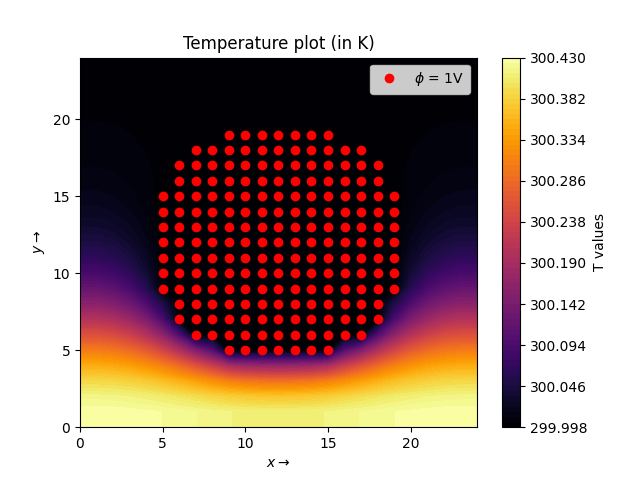
\includegraphics[scale = 0.75]{Figure_7.png}
    \label{fig:sample}
\end{figure}
\vspace*{-0.5cm}
\begin{center}
    The temperature is high in the region where the currents primarily exist and is
almost 300 K in the region where the currents are near zero. Hence, the
Laplace equation of temperature is satisfied properly    
\end{center}

\section{Results and Conclusions}
\begin{enumerate}
    \item The potential contour follows the boundary conditions properly and plot is also smooth
    \item The currents are primarily concentrated near the grounded edge. It makes
    sense that this is where the potential gradients exist in significant values.
    \item The temperature is higher than room temperature near the grounded region because the currents primarily exist there and hence, most of the
    Joule's heating take place there.
    \item The error initially is reducing steeply but reduces linearly after 500th
    iteration on the Semilogy plot.
    \item Judging by the time constant (Time constant = 1/B = 72.03), we can say
    this averaging method is not so preferable as the time taken by the error
    to settle is very high.
\end{enumerate}
\end{document}